% ============================================================
% 电路基础实验 —— 实验二 线性电路的线性特征 预习报告
% ============================================================

\documentclass[12pt]{ctexart}

% --- 宏包 ---
\usepackage{graphicx}
\usepackage{amsmath}
\usepackage{float}
\usepackage{booktabs}
\usepackage{siunitx}
\usepackage{caption}
\usepackage{subcaption}
\usepackage{enumitem}

\sisetup{per-mode=symbol}

\graphicspath{{./figures/}}

\usepackage[left=2.5cm, right=2.5cm, top=2.5cm, bottom=2.5cm]{geometry}

\setlength{\jot}{6pt}
\linespread{1.5}
\setlist{nosep}

\begin{document}

% ==================== 封面 ====================
\thispagestyle{empty}

\begin{center}
    \LARGE\textbf{第2次实验\ 验证线性电路的线性特征预习报告}

    \vspace{1cm}
    \normalsize
    组名：第7组\quad 姓名：郭浩然\quad 学号：2024303980
\end{center}

\vspace{1cm}

% ==================== 正文 ====================

% (10) 实验目的
\section{实验目的}

\begin{enumerate}[label=\arabic*.]
    \item 学习 LM317 三端可调节正电压稳压器的原理及其作为精密稳流器的使用方法。
    \item 验证线性电路的齐次性。
    \item 验证线性电路的叠加性。
\end{enumerate}

% (80) 实验原理
\section{实验原理}

\subsection{LM317 三端正电压稳压器}

LM317 是常见的三端可调节正电压稳压器，三个引脚分别为：引脚 1 ADJ（调整端）、引脚 2 \(V_{out}\)（输出端）、引脚 3 \(V_{in}\)（输入端）。封装形式与作为电流稳压器的典型接法分别如图~\ref{fig:lm317}(a)、(b) 所示。

将 LM317 与一只精密电阻 \(R_1\) 配合，可构成精密恒流源。其输出电流由内部 1.25\,V 基准电压决定：
\[
I_{out}=\frac{V_{ref}}{R_1}+I_{Adj}=\frac{1.25\,\text{V}}{R_1}
\]
正常工作范围为 \(10\,\text{mA}\le I_{out}\le 1.5\,\text{A}\)，调整端电流 \(I_{Adj}\) 通常远小于 \(I_{out}\)，可忽略不计。

\begin{figure}[H]
    \centering
    \begin{subfigure}[b]{0.32\textwidth}
        \centering
        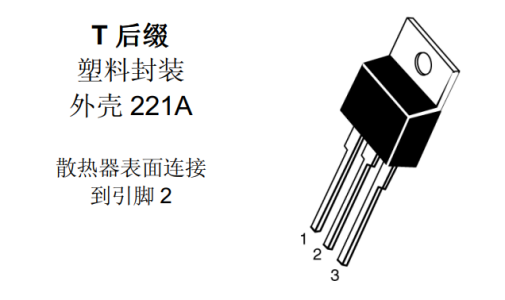
\includegraphics[width=\linewidth]{lm317_package.png}
        \caption{LM317 封装}
    \end{subfigure}
    \hfill
    \begin{subfigure}[b]{0.55\textwidth}
        \centering
        \includegraphics[width=\linewidth]{lm317_principle.png}
        \caption{LM317 作为精密电流稳压器}
    \end{subfigure}
    \caption{LM317 封装与电流稳压器接法}
    \label{fig:lm317}
\end{figure}

\subsection{齐次定理}

在线性电路中，当全部独立激励（独立电压源与独立电流源）同时增大或减小 \(K\) 倍（\(K\) 为常数）时，任一支路响应（电压或电流）也相应增大或减小 \(K\) 倍：
\[
y=f(x_1,x_2,\dots,x_n)\quad\Longrightarrow\quad Ky=f(Kx_1,Kx_2,\dots,Kx_n)
\]
本实验通过将电压源与电流源同时缩小至原值的一半，观察各支路电压、电流是否同步变化为原值的一半，以验证齐次性。

\subsection{叠加定理}

在线性电路中，当多个独立激励同时作用时，任一支路响应等于每个独立电源单独作用于线性电路时在该支路产生响应的代数和：
\[
y_1=f(x_1),\quad y_2=f(x_2)\quad\Longrightarrow\quad y_1+y_2=f(x_1+x_2)
\]
本实验中，分别测量电压源单独作用、电流源单独作用以及两者共同作用时各支路的电压与电流，比较"单独作用之和"与"共同作用"的实测值，以验证叠加性。注意：电压源单独作用时，电流源开路；电流源单独作用时，电压源用导线短接替代。

\subsection{实验电路与 Multisim 仿真}

实验电路的 Multisim 仿真接线如图~\ref{fig:multisim} 所示。由电压源 \(V_1=10\,\text{V}\)、辅助电源 \(V_2=18\,\text{V}\) 经 LM317AH 提供恒定电流，电阻 \(R_1=240\,\Omega\)、\(R_2=510\,\Omega\)、\(R_3=100\,\Omega\)、\(R_4=49.8\,\Omega\) 构成被测线性网络。仿真中通过万用表读取各支路电压、电流值，结果与齐次／叠加定理预期一致。

\begin{figure}[H]
    \centering
    \includegraphics[width=0.9\textwidth]{multisim_sim.png}
    \caption{实验电路 Multisim 仿真接线}
    \label{fig:multisim}
\end{figure}

% (10) 实验器件
\section{实验器件}

\begin{itemize}
    \item 面包板 \(\times 1\)
    \item 可编程直流电源 RIGOL DP832 \(\times 1\)
    \item 数字万用表 RIGOL DM858 \(\times 1\)
    \item LM317AH 芯片 \(\times 1\)
    \item 电阻：51\,\(\Omega\)\,\(\times 1\)、100\,\(\Omega\)\,\(\times 1\)、240\,\(\Omega\)\,\(\times 1\)、510\,\(\Omega\)\,\(\times 1\)
    \item 导线若干
\end{itemize}

\end{document}
